\begin{Exercise}[title=Lateral inhibition]
In this exercise we will create simple circuits that illustrate the concept of lateral inhibition, which is the 
capacity of an excited neuron to reduce the activity of its neighbors. This type of inhibition occurs primarily in 
visual process to increase the contrast and sharpness in visual response.

\Question{Create a circuit in Neuronify consisting of two passive excitatory and one passive inhibitory neuron, each 
connected to the same DC clamp. Adjust the current output of the DC clamp and see how the spiking pattern of the 
neurons changes.}

\Question{Create lateral connections from the inhibitory neuron to the excitatory neurons. You have now a very 
simple lateral inhibition circuit. How those these 
connections affect the activity in the excitatory neurons?}
   
\Question{Make the connections in the network shown below such that the same spiking patterns are as in the 
figure. You are allowed to adjust the 
\emph{stimulation output} property of the cells.}
      
\end{Exercise}

    
\begin{figure}[h!]
  \centering
    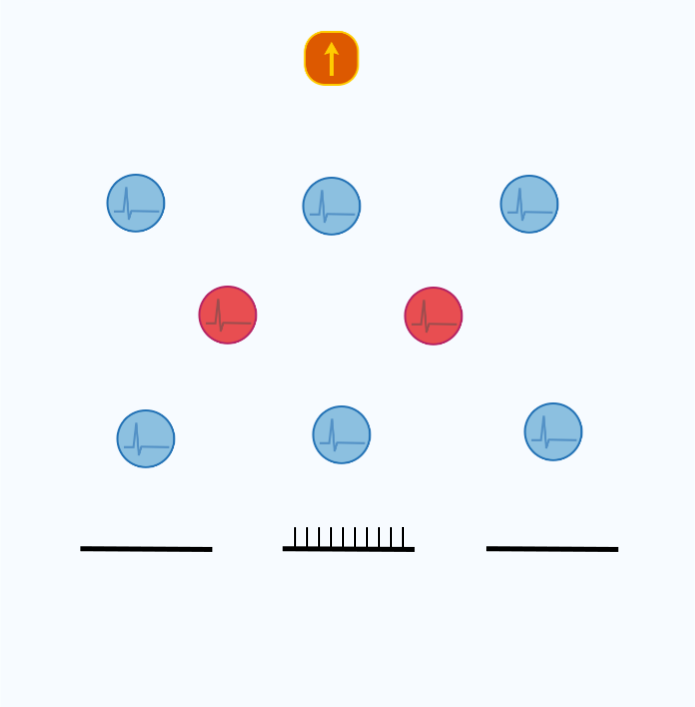
\includegraphics[width=0.5\textwidth]{figures/lateralInihibition.png}
      \caption{Lateral inhibition network.}
\end{figure}